\subsection{Design Diagrams} \label{desSysDiag}
%use-case diagram
\begin{figure}[h!]
  \begin{tikzpicture}
    \begin{umlsystem}{Robot Functions}
      \umlusecase[x=0,y=0, name=useState]{Set State}
      \umlusecase[x=0,y=-1,name=useScan]{Scan Floor}
      \umlusecase[x=0,y=-2,name=useMove]{Move Around}
      \umlusecase[x=0,y=-3,name=useRotate]{Rotate}
      \umlusecase[x=0,y=-4,name=useSwap]{Swap Motor Strength}
      \umlusecase[x=0,y=-5,name=useConn]{Connect to other Robots} 
    \end{umlsystem}

    \umlactor[x=-6,y=-3.5]{User}
    \umlactor[x=6,y=-3.5]{Robot}

    \umlassoc{User}{useState}
    \umlassoc{Robot}{useState}
    \umlassoc{Robot}{useScan}
    \umlassoc{Robot}{useMove}
    \umlassoc{Robot}{useRotate}
    \umlassoc{Robot}{useSwap}
    \umlassoc{Robot}{useConn}
  \end{tikzpicture}
  \caption{Use Case Diagram for proposed software solution}
  \label{desSysUse}
\end{figure}

%Class Diagram
\begin{figure}[h!] 
  \begin{tikzpicture}
    \begin{umlpackage}{StiCo Algorithm}
      \umlclass[x=0,y=0]{Movement}{
        headMotorPower : short* \\ tailMotorPower : short* \\ tempPower : short*
      }{
        setMovementSpeed(short*, short*) : void \\ swapMovementSpeed(short*, 
        short*) : void
      }
      \umlclass[y=5]{Light}{
         lightStrength : short* \\ lightStorage : short**
       }{
         setLightStrength(short*) : void \\ scanLight(short**) : void
       }
       \umlclass[x=5,y=5]{Main}{}{}
       
       \umlimport{Main}{Movement}
       \umlimport{Main}{Light}
    \end{umlpackage}
  \end{tikzpicture}
  \caption{Class Diagram for StiCo Implementation}
  \label{desSysClassStiCo}
\end{figure}


%Traditional Design
%data dictionaries
\begin{landscape}
  \subsubsection{Data Dictionary}
  \begin{tabular}{| p{5cm} | p{4cm} | p{3cm} | p{6cm} |}
    \hline
    Attribute name & Description & Found in entity & Occurrence\\
    \hline
    lightStrength  & Stores current agent's light intensity & Light    &
    Whenever the agent needs to change light intensity              \\
    \hline
    lightStorage   & Stores localised light intensity       & Light    &
    When the agent scans the floor for localised messages           \\
    \hline
    headMotorPower & Stores left wheel movement strength    & Movement &
    When movement speed is modified or change in rotation direction \\
    \hline
    tailMotorPower & Stores right wheel movement strength   & Movement &
    When movement speed is modified or change in rotation direction \\
    \hline
    tempPower      & Stores headMotorPower                  & Movement &
    Used each time the robot needs to change rotational direction   \\
    \hline
    currentPos     & Stores agent's position                & Movement &
    Used during HybaCo execution.  Used to calculate moving decision\\
    \hline  
  \end{tabular}
\end{landscape}
\clearpage

\begin{figure}
  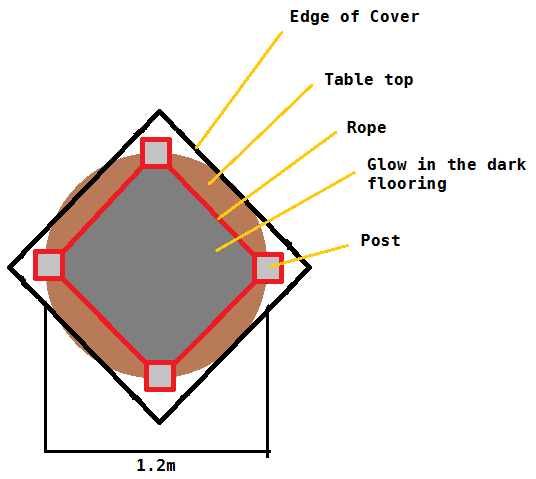
\includegraphics[scale=0.7]{img/ArenaTopDown.png}
  \caption{Top down view of the proposed dark room} \label{desSysTopImg}
\end{figure}
\begin{figure}
  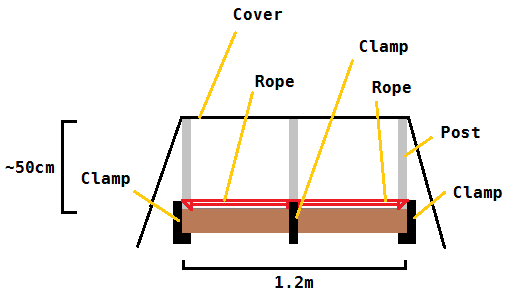
\includegraphics[scale=0.7]{img/ArenaSideView.png}
  \caption{Side view of the proposed dark room} \label{desSysSideImg}
\end{figure}
\clearpage

\subsection{Project Pseudo-code}
%pseudo code of main methods
\begin{algorithm}
  \caption{StiCo Algorithm\cite{Ranjbar-Sahraei2012Demo} }
  \label{desSysPseuStiCo}
  \begin{algorithmic}[1]
    \Require Each robot can deposit/detect pheromone trails \par
    \State Initialise: Choose circling direction (CW/CCW)
    \Loop
    \While{ (no pheromone is detected) }
    \State Circle around
    \State deposit Pheromone
    \EndWhile
    \If{ (interior sensor detects pheromone) }
    \State Reverse the circling direction
    \Else
    \While{ (pheromone is detected) }
    \State Rotate
    \EndWhile
    \EndIf
    \EndLoop
  \end{algorithmic}
\end{algorithm}

\subsection{Rope-length Algorithm}
\begin{algorithm}
  \caption{Rope Length Calculator (Measurements in centimetres) }
  \label{desSysRope}
  \begin{algorithmic}[1]
    \State $ Edge = 3(\sqrt{2(r^{2} ) } ) + 2 $
    \Comment Multiplying by 3 is due to tripling the rope over
    \State $ WrappedPost = (postPerimeter \times 2) + 2 $
    \Comment Trailing 2's are for securing the rope
    \State $ TotalRequiredRope = 4(Edge + WrappedPost) $
  \end{algorithmic}
\end{algorithm}
\clearpage

\begin{landscape}
%Modified Gantt chart
\subsection{Gantt Chart}
\begin{ganttchart}[y unit chart=0.9cm]{24}{24}
  \gantttitle{2015}{12} \gantttitle{2016}{12} \\
  \gantttitlelist{1,...,12}{1} \gantttitlelist{1,...,12}{1} \\
  \ganttgroup{Req.}{1}{4} \\
  \ganttbar[name=reqRes]{Research}{1}{3} \\
  \ganttbar[name=reqWrite]{Req. Write Up}{4}{4} \\
  \ganttlink{reqRes}{reqWrite}
  
  \ganttgroup{Des.}{5}{8} \\
  \ganttbar[name=desArena]{ArenaBlueprints}{5}{7} \\
  \ganttbar[name=desAlSearch]{AlgorithmResearch}{5}{6} \\
  \ganttbar[name=desPseudo]{PseudoCode}{7}{7} \\
  \ganttmilestone[name=milDesFin]{Des. Content Finished}{7} \\
  \ganttbar[name=desWrite]{Des. Write Up}{8}{8} \\
  \ganttlink{desArena}{milDesFin}
  \ganttlink{desAlSearch}{desPseudo}
  \ganttlink{desPseudo}{milDesFin}
  \ganttlink{milDesFin}{desWrite}
  
  \ganttgroup{Imp.}{9}{20} \\
  \ganttbar[name=impArena]{Build Arena}{9}{11} \\
  \ganttbar[name=impFamiliar]{Coding Robot famil.}{10}{11} \\
  \ganttmilestone[name=milArenaFin]{Built Dark Room}{11} \\
  \ganttbar[name=impBasicCode]{Basic Code}{12}{14} \\
  \ganttbar[name=impAdvCode]{Advanced Code}{15}{17} \\
  \ganttmilestone[name=milCodeFin]{Finished Coding}{17} \\
  \ganttbar[name=impRefactor]{Refactor}{18}{18} \\
  \ganttbar[name=impWrite]{Imp. Write Up}{19}{20} \\
  \ganttlink{impArena}{milArenaFin}
  \ganttlink{impFamiliar}{milArenaFin}
  \ganttlink{milArenaFin}{impBasicCode}
  \ganttlink{impBasicCode}{impAdvCode}
  \ganttlink{impAdvCode}{milCodeFin}
  \ganttlink{milCodeFin}{impRefactor}
  \ganttlink{milCodeFin}{impWrite}
\end{ganttchart}
\end{landscape}
\clearpage
